% Ubah judul dan label berikut sesuai dengan yang diinginkan.
\section{Arsitektur}
\label{sec:arsitektur}

% Ubah paragraf-paragraf pada bagian ini sesuai dengan yang diinginkan.

\subsection{Perancangan Sistem Deteksi Helm Keselamatan Kerja}
\label{subsec:perancangansistemdeteksihelmkeselamatankerja}

Sistem deteksi yang dibuat untuk Deteksi Helm Keselamatan kerja sendiri dikembangkan dari sistem deteksi yang sudah ada dari YOLOv5 dengan beberapa perubahan yang disesuaikan khusus untuk judul ini. 

Sistem yang dibuat direncanakan akan dijalankan di komputer yang sudah terinstall Python dan framework PyTorch atau ONNX dimana merupakan format yang dihasilkan dari training sebelumnya.

Sistem nya akan dibuat sebagai file script python yang dapat di run dan dapat menerima beberapa parameter : ukuran gambar, sumber input, dan bobot atau weight yang akan digunakan. 
Input yang dapat digunakan dengan script yang dibuat dapat dilakukan dalam bentuk gambar, file video, link youtube, link stream, dan feed camera dengan basis dari script detect.py dari YOLOv5. Tetapi, yang akan digunakan sebagai default nanti adalah feed dari kamera atau webcam yang tersedia di hardware yang digunakan untuk menjalankan inference. Ukuran atau resolusi gambar yang diterima sebagai ukuran default yaitu 640x640. 

Untuk kasus jika input berupa gambar tunggal, gambar tersebut akan digunakan untuk inference melalu model yolov5 dengan bobot yang sudah dibuat sebelumnya lalu hasil inference yolov5 akan menghasilkan beberapa output. Tetapi untuk sistem yang akan dijalankan akan memanfaatkan feed dari camera atau webcam secara realtime sehingga akan dilakukan inference untuk tiap frame yang masuk dari input webcam.

Output yang dikeluarkan dari hasil inferensi menggunakan yolov5 yaitu xcenter, ycenter, width , height, confidence, dan class. Untuk keperluan menampilkan bounding box akan menggunakan xcenter, ycenter, width, dan height yang didapatkan dari output inference yang lalu dilengkapi dengan menampilkan nama class dan confidence score dari inferencenya. 

Untuk fungsi trigger alarm jika terdeteksi adanya orang yang tidak menggunakan helm, untuk hasil output yang dihasilkan dari inference satu frame akan dicheck sekiranya mengandung class “no\textunderscore helmet” yang jika terpenuhi akan  menjalankan perintah untuk mengeprint “NO HELMET DETECTED” pada display dan menjalankan audio alarm. 


% Contoh input gambar pada kolom.
\begin{figure} [ht]
  \centering
  % Ubah sesuai dengan nama file gambar dan ukuran yang akan digunakan.
  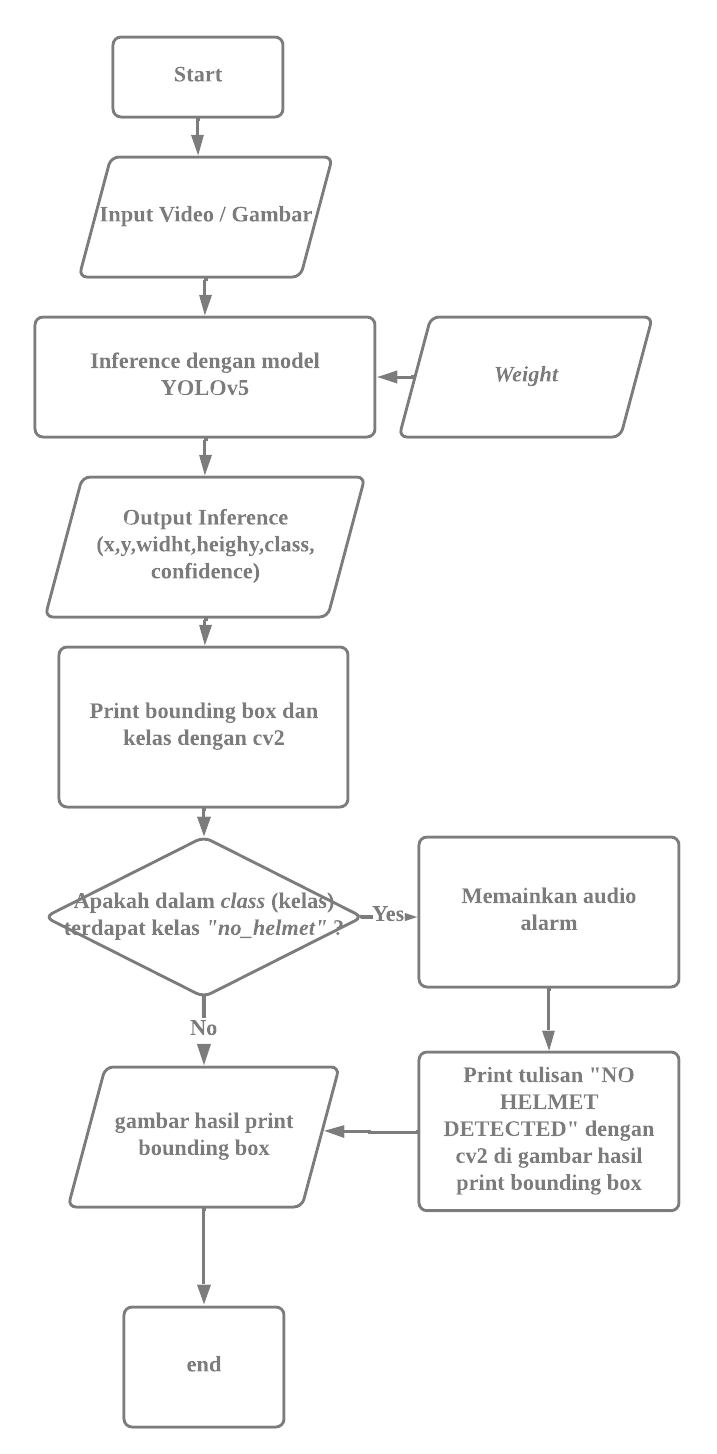
\includegraphics[width=0.4\textwidth]{gambar/flowchart_sistem.png}

  % Ubah sesuai dengan keterangan gambar yang diinginkan.
  \caption{flowchart Sistem}
  \label{fig:cetakbiru}
\end{figure}

\subsection{Model YOLOv5}
\label{subsec:yolov5model}

YOLOv5 merupakan versi pembaruan dari YOLO yang dicetuskan pada tahun 2020 oleh Glenn Jocher \cite{glenn_jocher_yolov5}. Berdasarkan dari \emph{repository} Github untuk YOLOv5 oleh Glenn Jocher, struktur jaringan dari YOLOv5 dibagi menjadi 3 bagian utama yaitu modul \emph{Backbone}, \emph{Neck}, dan \emph{Head}.
Seperti yang dapat dilihat di Gambar \ref{fig:yolov5network} Struktur jaringan dari YOLOv5 ini dimulai dari modul \emph{Backbone} dimana dilewati pertama oleh input gambar untuk mengekstrak fitur - fitur dari gambar yang strukturnya berbasis dari struktur \emph{Focus}, \emph{Bottleneck CSP (Cross Stage Partinal Networks)}, dan \emph{Spatial Pyramid Pooling (SPP)}.
Hasil ekstraksi fitur dari \emph{Backbone} lalu digunakan untuk menghasilkan \emph{feature pyramid} di modul \emph{Neck} yang merupakan struktur yang berbasis dari PANet (\emph{Path Aggregation Network}).
Lalu terakhir di Modul \emph{Head} dilakukan penampilan \emph{bounding box} yang meliputi beberapa informasi yaitu : kelas, koordinat, dan \emph{confidence score}.

\begin{figure} [ht]
  \centering
  % Ubah sesuai dengan nama file gambar dan ukuran yang akan digunakan.
  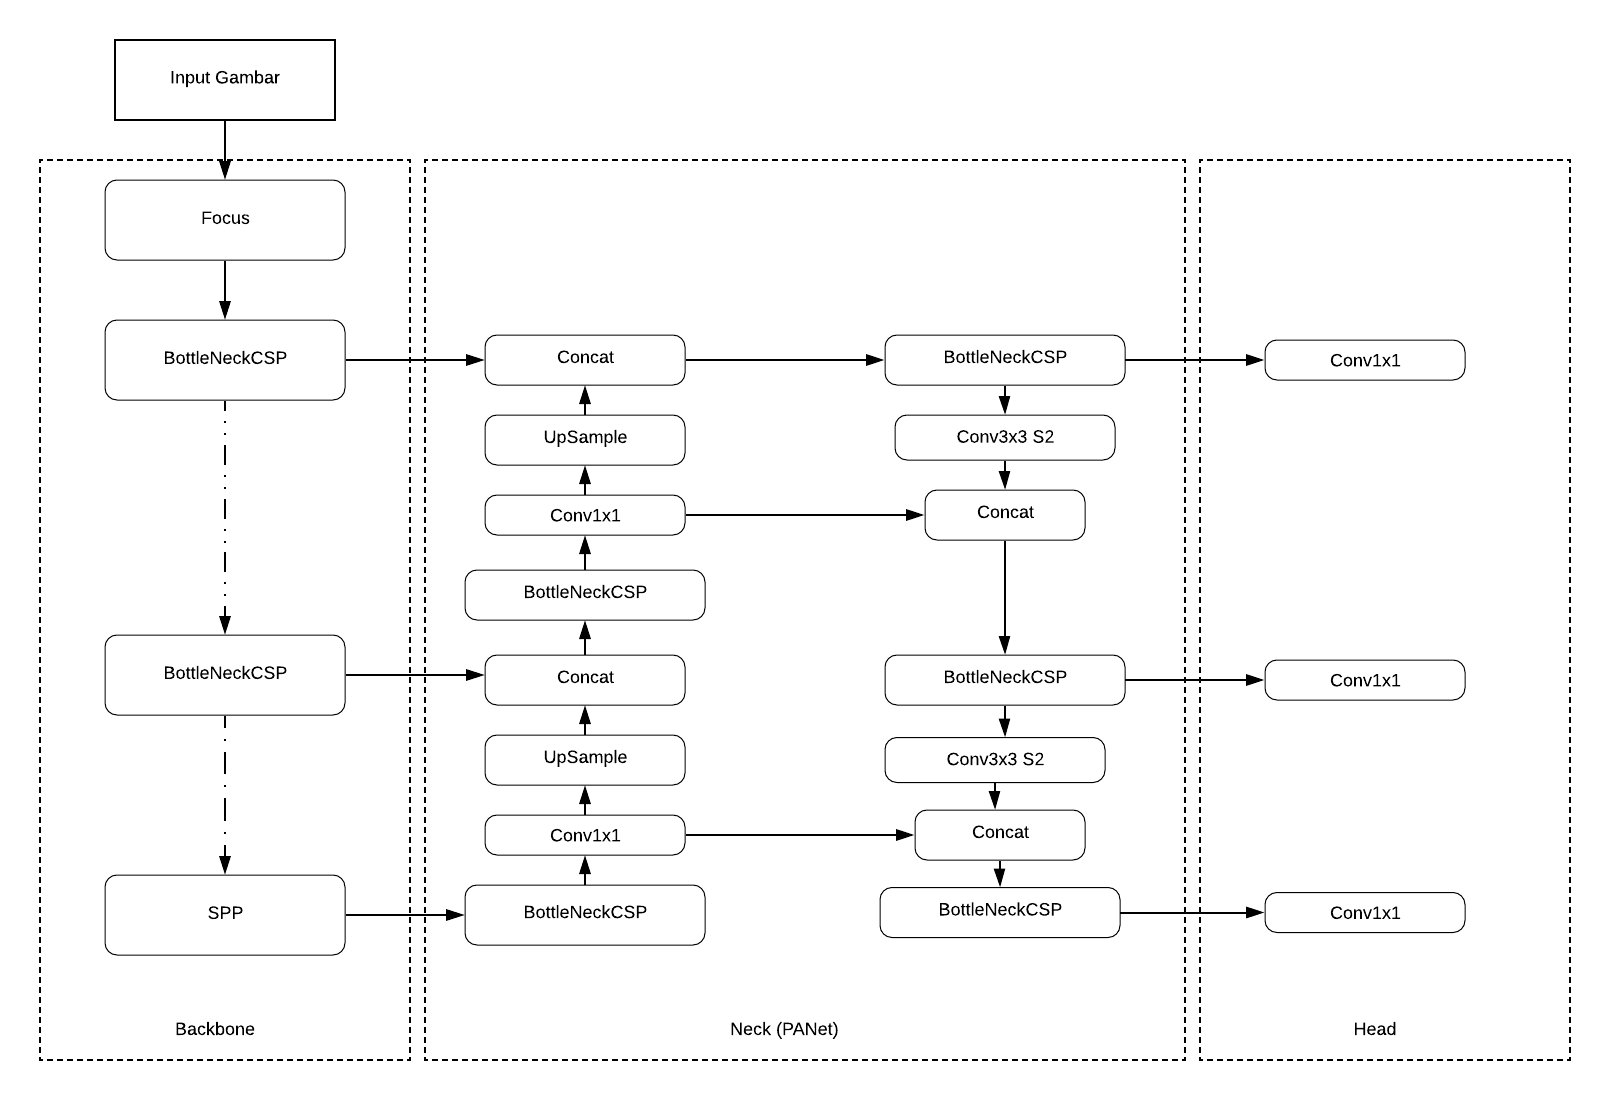
\includegraphics[width=0.4\textwidth]{gambar/yolov5 structure.png}

  % Ubah sesuai dengan keterangan gambar yang diinginkan.
  \caption{YOlov5}
  \label{fig:yolov5s}
\end{figure}

% Contoh pembuatan tabel.
\begin{table}
  \caption{Contoh tabel sederhana}
  \label{tab:tabelsederhana}
  \centering
  \begin{tabular}{lll}
    \toprule
    Heading1 & Heading2 & Heading3  \\
    \midrule
    One      & Two      & Three     \\
    Four     & Five     & Six       \\
    \bottomrule
  \end{tabular}
\end{table}

% Contoh pembuatan potongan kode.
\begin{lstlisting}[
  language=C++,
  caption={Program halo dunia.},
  label={lst:halodunia}
]
#include <iostream>

int main() {
    std::cout << "Halo Dunia!";
    return 0;
}
\end{lstlisting}

\lipsum[12]

% Contoh pembuatan daftar.
\begin{enumerate}
  \item \lipsum[13][1-4]
  \item \lipsum[13][5-8]
  \item \lipsum[13][9-12]
\end{enumerate}

\lipsum[14-15]
